%%%% hw3-reqdoc.team3.tex
%%%% Requirements Documentation for sQuire
%%%% Due on BBLearn before 10pm on Tuesday 2/9/2016

\documentclass[11pt]{report}

\usepackage{graphicx}
\usepackage{wrapfig}
%\graphicspath{ {images/} }

\marginparwidth 0.5in 
\oddsidemargin 0.25in 
\evensidemargin 0.25in 
\marginparsep 0.25in
\topmargin 0.0in 
\textwidth 6in \textheight 8.5in

\title{Squire: A Collaborative Software Development Tool}
\author{jank6275, mora5651, boss2849, bolt1003, gall7417, brec9824, snev7821, mars2681}

\begin{document}

\maketitle

\tableofcontents

\chapter{Introduction}

\section{Program Premise}
    \begin{wrapfigure}{r}{0.9\textwidth}
      \begin{center}
        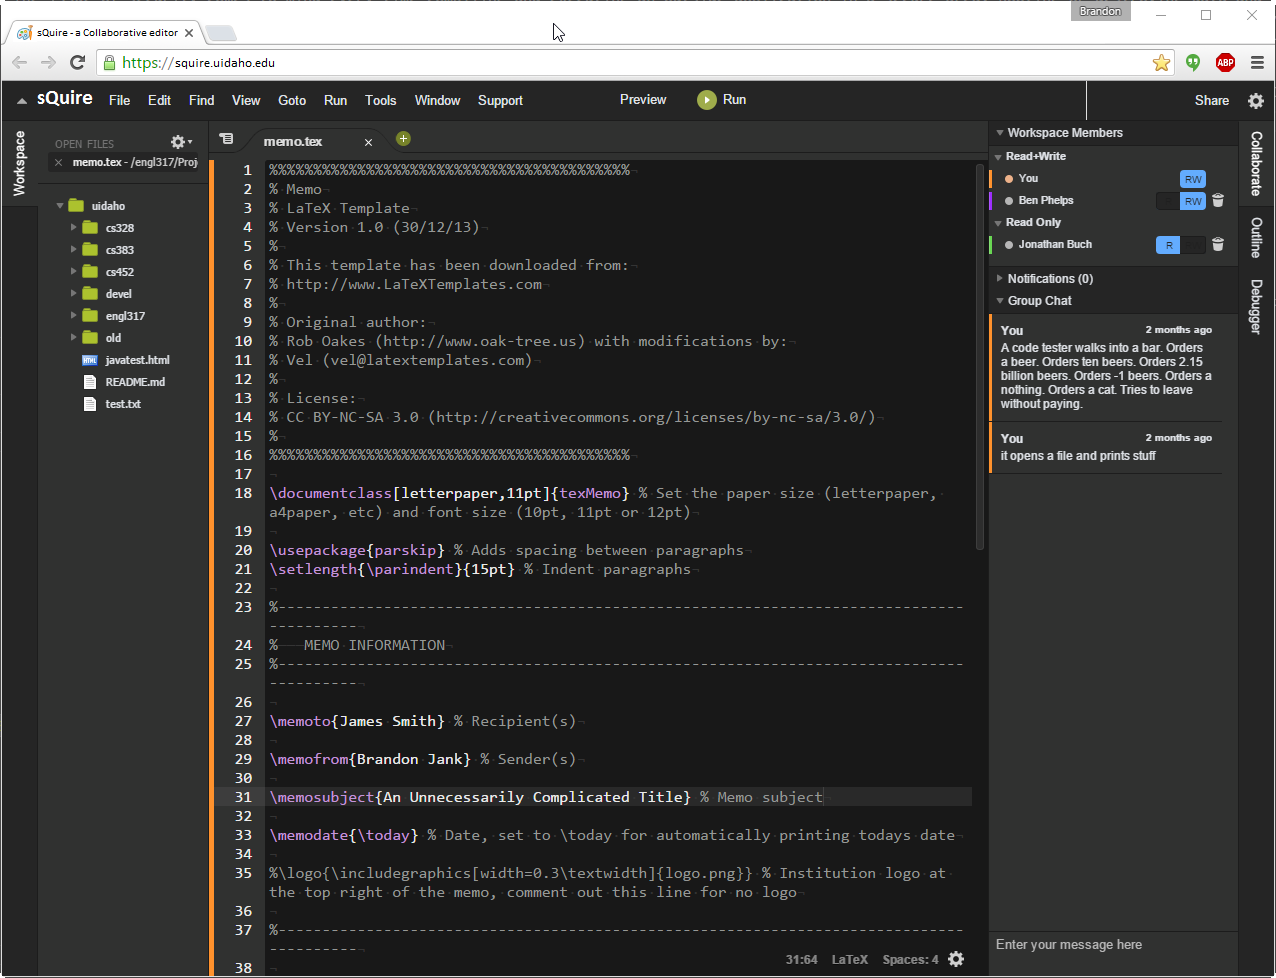
\includegraphics[width=0.7\textwidth]{squire}
      \end{center}
      \caption{Squire is a web-based collaborative software development environment with a project development center. Squire will allow multiple users to edit files and communicate in real time. Projects can be ``stubbed'' out by a user and then other users can join and/or vote to support for their favorite projects. After a certain amount of support, planning, and documentation is reached for a project, the project becomes a fully fleged project and then community development can start. Think ``kickstarter for code'' where people pledge their help with the project and not just financial support.}
    \end{wrapfigure}


\chapter{Class Diagrams}
The "detail" subteams should show as much detail about their assigned classes' associations, attributes, and methods as is known at this time. Edits of all kinds can be made later on.
Every UML diagram should have 1+ author name(s) in a small font, and be accompanied by a supporting "diagram dictionary": a section of prose text that defines the classes and user-defined associations, and clarifies any ambiguities or tricky sections of the diagram. All UML diagrams should be reviewed for completeness and accuracy by at least one other team member; add "reviewed by XXX" in a small font after the author name(s) in the diagram. Be "egoless" and take criticism seriously, fixing or adding things can help your grade. Within your team, check to make the diagrams mutually consistent and stylistically consonant. Adopt standards for fonts and such within your team.



\section{Overview ()}
Each team should assign one additional "overview" subteam to draw one or more higher-level overview class diagrams showing the aggregated big picture, with more classes and associations showing but class class detail. This could be one giant diagram, or separate diagrams for inheritance, aggregation, and user-defined associations, or provide an overview along some other structured lines.



\section{Authentication (mora5651)}



\section{Project Management (bolt1003)}



\section{Project Ideas (mars2681)}



\section{Settings - Preferences \& Profile (brec9824)}



\section{Compiler (boss2849)}



\section{Syntax (gall7417)}



\section{Communication (jank6275)}
    \begin{wrapfigure}{r}{0.9\textwidth}
        \begin{center}
            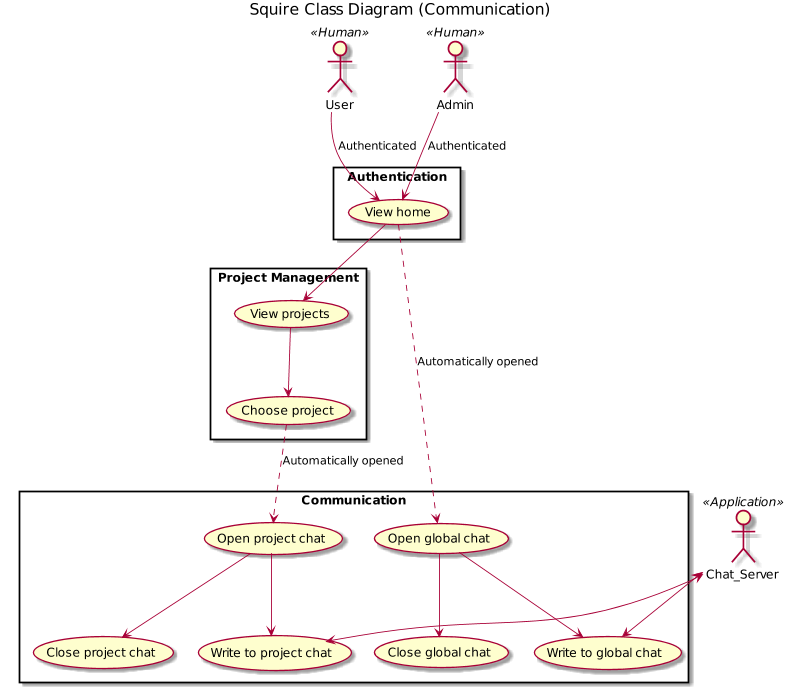
\includegraphics[width=0.7\textwidth]{diagrams/communication-jank6275}
        \end{center}
        \caption{Squire is a web-based collaborative software development environment with a project development center. Squire will allow multiple users to edit files and communicate in real time. Projects can be ``stubbed'' out by a user and then other users can join and/or vote to support for their favorite projects. After a certain amount of support, planning, and documentation is reached for a project, the project becomes a fully fleged project and then community development can start. Think ``kickstarter for code'' where people pledge their help with the project and not just financial support.}
    \end{wrapfigure}


\section{Project File Editor (snev7821)}
    \includegraphics[scale=0.7]{diagrams/ProjectFileEditor-snev7281}
    The project File Editor is simply the file system for Squire. It provides basic read/write permission for any user related to a project. Only admins of a project may move project files, delete old files, and create new files.


    
\end{document}